\documentclass{report}

%%Ableitungsverknüpfung

\usepackage[ngerman]{babel}
\newcommand{\la}{\lambda}
\newcommand{\dl}{\Delta \lambda}
\newcommand{\Ra}{\Rightarrow}
\usepackage[utf8]{inputenc}
\usepackage[T1]{fontenc}
\usepackage{pgfplots}
\usepackage{xcolor}
%\usepackage{ntheorem}
\usepackage{chngcntr}
\usepackage{amsmath}
\usepackage{mathrsfs}
\usetikzlibrary{arrows}
\usepackage{mathtools}
\pgfplotsset{compat=1.15}
\usepackage{amssymb}
\usepackage{amsthm}
\usepackage{geometry}
\geometry{tmargin=25mm, bmargin=20mm, lmargin=50mm, rmargin=35mm}
\usepackage{mathtools}
\usepackage{drawmatrix}
%\theoremstyle{defintion}
\newtheorem {satz}{Satz}
\usepackage{pdfpages}
\bibliographystyle{abbrv}
\usepackage{lastpage}
\usepackage[fixFPpow]{tabularcalc}
\usepackage{xcolor}
\newtheorem{geg}{Gegeben}
\usepackage{graphicx}
\usepackage{hyperref}
\graphicspath{Bilder/}
\usepackage{chngcntr}
\usepackage{mathrsfs}

\usepackage{thmtools}

\usepackage[font={small,sf}]{caption}

\usepackage{svg}

%\renewcommand{\listtheoremname}{Definitionsverzeichnis}

\renewcommand{\d}{\text{d}}
\newcommand{\Mod}[1]{\ (\mathrm{mod}\ #1)}
\newcommand{\R}{\mathbb{R}}
\newcommand{\N}{\mathbb{N}}
\newcommand{\dx}{\; \text{d} x}
\newcommand{\x}{\cdot}
\newcommand{\red}{\color{red}}
\newcommand{\green}{\color{olive}}
\newcommand{\blue}{\color{blue}}
\newcommand{\black}{\color{black}}
\newcommand{\nt}{\notag}
\newcommand{\dis}{b^2-4ac}
\newcommand{\trennl}{\noindent\rule[0.5ex]{\linewidth}{1.5pt}}
\newcommand{\btrennl}{\noindent\rule[0.5ex]{\linewidth}{3pt}}
\newcommand{\abc}{\frac{-b \pm \sqrt{b^2-4ac}}{2a}}
\usepackage{multicol}
\usepackage{mdframed}
\usepackage{fancyhdr}
\pagestyle{fancy}

\fancyhead[L]{\sffamily\bfseries\nouppercase\leftmark}
\fancyhead[R]{\sffamily Lukas Semrau}
\fancyfoot[C]{\thepage}

\rfoot{}
%\lfoot{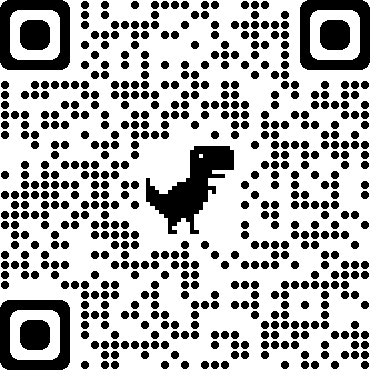
\includegraphics[scale=0.05]{bilder/qr.png}}

\definecolor{ffqqtt}{rgb}{1,0,0.2}
\definecolor{qqqqff}{rgb}{0,0,1}
\definecolor{qqwuqq}{rgb}{0,0.39215686274509803,0}
\usetikzlibrary{quotes,angles}
\theoremstyle{definition}
\newtheorem{aufgabe}{Aufgabe}[section]

\theoremstyle{definition}
\newtheorem{losung}{Lösung}[section]

\usepackage{url}



\newtheoremstyle{an} % name
    {\topsep}                    % Space above
    {\topsep}                    % Space below
    {\itshape}                   % Body font
    {}                           % Indent amount
    {\itshape\sffamily}                   % Theorem head font
    {.}                          % Punctuation after theorem head
    {.5em}                       % Space after theorem head
    {}  % Theorem head spec (can be left empty, meaning ‘normal’)

\theoremstyle{an}
\newtheorem{anm}{Anmerkung}[section]

\renewcommand{\theequation}{\arabic{section}.\arabic{equation}}
\renewcommand{\qedsymbol}{$\blacksquare$}

\usepackage{titlesec}
\titleformat{\chapter}{ \scshape\centering\huge \bfseries \sffamily}{\thechapter\quad }{}{}

\usepackage{roboto}

%\titleformat{\section}{\centering\Large \bfseries \sffamily }{\thesection\quad }{}{}

\counterwithin*{equation}{section}


\newtheoremstyle{lem} % name
    {\topsep}                    % Space above
    {\topsep}                    % Space below
    {\itshape}                   % Body font
    {}                           % Indent amount
    {\scshape\sffamily}                   % Theorem head font
    {.}                          % Punctuation after theorem head
    {.5em}                       % Space after theorem head
    {}  % Theorem head spec (can be left empty, meaning ‘normal’)

\theoremstyle{lem}
\newtheorem{lemma}{Lemma}[section]


\usepackage{forest}
\usepackage{enumitem}
\usepackage{verbatim}

\newcommand{\re}[1]{\textsf{#1}}


\newtheoremstyle{def} % name
    {\topsep}                    % Space above
    {\topsep}                    % Space below
    {}                   % Body font
    {}                           % Indent amount
    {\bfseries\sffamily}                   % Theorem head font
    {.}                          % Punctuation after theorem head
    {.5em}                       % Space after theorem head
    {}  % Theorem head spec (can be left empty, meaning ‘normal’)

\theoremstyle{def}
\newmdtheoremenv{defi}{Definition}[section]

\theoremstyle{def}
\newmdtheoremenv{merk}{Merke}[section]

\setlength{\marginparwidth}{4cm}
\renewcommand{\theequation}{\textsf{\arabic{chapter}.\arabic{section}.\arabic{equation}}}
\begin{document}
	\title{Mathematik ab der neunten Jahrgangsstufe}
	\author{Lukas Semrau}
	\date{Schuljahr 2020/21}
	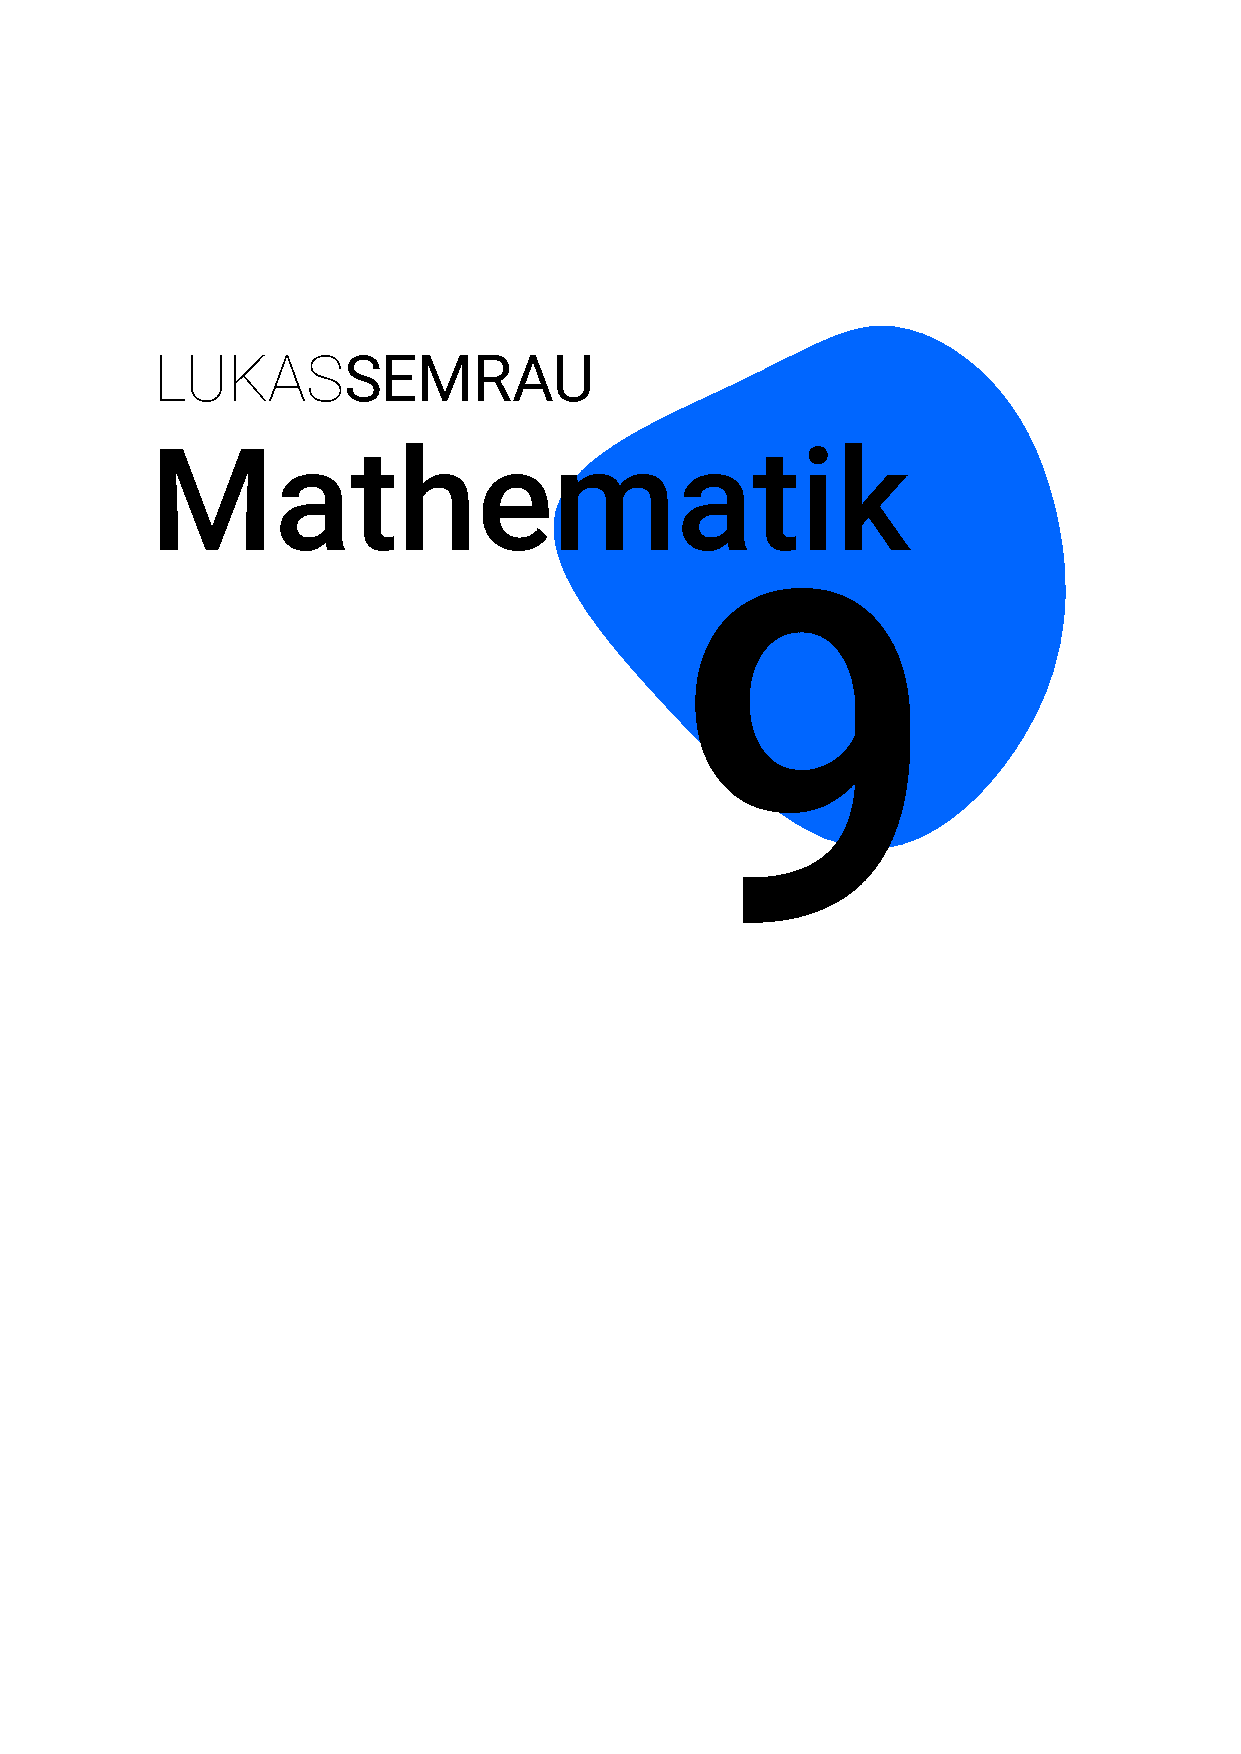
\includepdf[]{bilder/title.pdf}
	\tableofcontents
	\listoffigures \bigskip
	\begin{anm}
		Interaktive Materialien können unter \url{www.linktr.ee/mathematik9} aufgerufen werden.
		\begin{figure}[h]
			\centering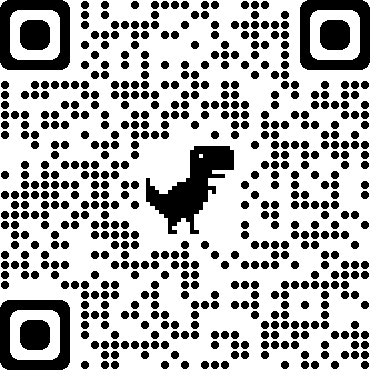
\includegraphics[scale=0.3]{bilder/qr.png}
		\end{figure}
	\end{anm}

	
	\begin{anm}[Kontakt]
		Bei Fragen ist sich an \url{lukas@lukas-semrau.de} zu wenden, das Skript lässt sich auf meiner Website \url{www.lukas-semrau.de} herunterladen.
	\end{anm}
	
	\pagebreak
%	\listoftheorems[ignoreall,show={defi,lemma,merk,satz}]
	\chapter{Reelle Zahlen}
 	\section{Quadratwurzel}
	\begin{defi}[Quadratwurzel]
		Für $a \geq 0$ ist $\sqrt{a}$ diejenige nicht negative Zahl, deren Quadrant $a$ ergibt. $\sqrt{a}$ heisst \textbf{Quadratwurzel}, $a$ heit \textbf{Radikant}.
		\begin{align}
			\sqrt{a^2}=\left| a \right|
		\end{align}
	\end{defi}
	
	Dabei sind folgende Dinge zu beachten:
	\begin{enumerate}
		\item $\sqrt{a}$ ist nach Definition eine eindeutig bestimmte Zahl, die grösser oder gleich null ist. \reversemarginpar \marginpar{\begin{flushleft}
				$-\sqrt{81}=-9$ aber $\sqrt{-81}=$undef. \end{flushleft}}
		\item Man kann nur aus positiven Zahlen $x\in \R^+_0$ die Quadratwurzel $\sqrt{x}$ ziehen, denn beim Quadrieren einer Zahl ergeben sich niemals negative Zahlen. Für $y\in \R$ gilt
		\begin{align}
			y^2\in \R^+_0
		\end{align}
	\end{enumerate}
	\begin{anm}
		Man könnte sagen, dass die Wurzel die Umkehrung des Quadrierens ist. \quad $y=x^2 \Ra x=\sqrt{y}$ \quad Bei dieser Gleichung muss man keine Betragsstriche setzen, da man hier die Wurzel als \textit{Umkehrung des Quadrierens} benutzt.  
	\end{anm}
	\section{Reelle Zahlen}
	\subsection{Unzugänglichkeit der rationalen Zahlen}
	\begin{satz}[Irrationalität von $\sqrt{2}$]
		Die Wurzel aus 2 $\sqrt{2}$ lässt sich nicht als teilerfremden Bruch $\sqrt{2}=\frac{p}{q}$ mit $p,q\in \mathbb{Q}$ darstellen.
	\end{satz}
	\begin{proof}[Beweis von Euklid.]
		Im folgenden wird ein Beweis durch Widerspruch vollzogen, d.h. wir nehmen an, die zu widerlegende Aussage sei wahr und finden dann einen Widerspruch.\\
		Sei $\sqrt{2}=\frac{p}{q}$ mit teilerfremden Zahlen $p,q\in \mathbb {Q}$, dann kann man dies zu 
		\begin{align}
			2&=\frac{p^2}{q^2} \\
			2q^2&=p^2
		\end{align} umformen, d.h. $p^2$ ist durch 2 teilbar.
		\begin{lemma}[Teilbarkeit von Zahl und Quadratzahl]
			Ist eine Zahl $a^2$ durch $b$ teilbar, so ist auch eine Zahl $a$ durch $b$ teilbar.
		\end{lemma}
		
	 Daraus folgt, dass auch $p$ durch 2 teilbar ist. Sei $p=2r$. Dies kann man zu 
	 \begin{align}
	 	q^2=2r^2
	 \end{align}
 	umformen, d.h. $q^2$ und $q$ ist durch 2 teilbar.\\
 	Dies stellt einen Widerspruch dar, da $p$ und $q$ durch 2 teilbar sind, der Bruch aber vollständig gekürzt sein soll.
 \end{proof}
 	\subsection{Die Menge der reellen Zahlen}
 	\begin{defi}[Reelle Zahlen]
 		Zahlen, die sich weder durch endliche noch durch periodische (unendliche) Dezimalbrüche darstellen lassen, heissen \textbf{irrationale Zahlen} $\mathbb{I}$. Sie lassen sich nicht mit beliebiger Genauigkeit durch rationale Zahlen annähern. \\
 		Rationale und irrationale Zahlen bilden bilden zusammen die Menge der \textbf{reellen Zahlen} $\R$. (s. Abb. \ref{fig:mengen}) 
 		\begin{align}
 			\mathbb{Q} \cup \mathbb{I}=\R
 		\end{align}
 	\end{defi}
	\begin{figure}[h]
			\centering
			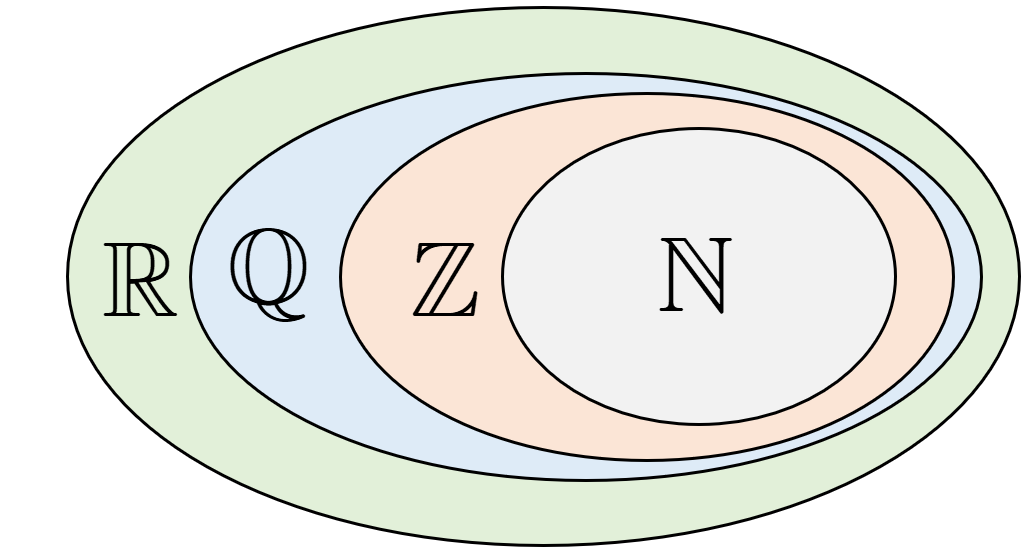
\includegraphics[width=0.7\linewidth]{bilder/Mengen2.png}
			\caption[Alle Mengen im Überblick]{Alle Mengen im Überblick}
			\label{fig:mengen}
	\end{figure}
	\section{Rechnen mit Quadratwurzeln}
	\begin{defi}[Quadratzahlen unter der Quadratwurzel]
		\begin{align}
			&\text{Für}\; a\geq0 \; \text{gilt}:& \sqrt{a^2}&=a \\
			&\text{Für}\; a\leq0 \; \text{gilt}:& \sqrt{a^2}&=-a
		\end{align}% \marginpar{\begin{flushleft}
		%	Bsp.: $\sqrt{(-3)^2}=-(-3)=3$
	%\end{flushleft}} 
	\end{defi}
	\begin{defi}[Multiplikation-/ Divisionsregel]
		Für $a,b\geq 0$ und in \eqref{eq:eq1} $b\neq 0$ gilt:
		\begin{align}
			&\text{Die Multiplikationregel}:& \sqrt{ab}&=\sqrt {a} \x \sqrt{b} \label{eq:eq2} \\
			&\text{Die Divisionsregel}:& \sqrt{\frac ab}&=\frac{\sqrt {a}}{\sqrt{b}} \label{eq:eq1}
		\end{align}
	\end{defi} \pagebreak
	\begin{proof}[Beweis zu \eqref{eq:eq2}]
	$\sqrt{a\x b}$ ist die (positive) Zahl, die beim Quadrieren $a\x b$ ergibt. Es ist also zu zeigen, dass auch beim quadrieren von $\sqrt a \x \sqrt b$ der Term $a\x b$ ergibt:
	\begin{align}
		\left(\sqrt{a}\x \sqrt{b}\right)^2= \left(\sqrt a\right)^2 \x \left( \sqrt b \right)^2=ab
	\end{align}
	Der Beweis zu \eqref{eq:eq1} verläuft analog, da $\frac ab =a\x b^{-1}$
	\end{proof}
	\begin{anm}
		Es gilt $\sqrt a +\sqrt b \neq \sqrt{a+b}$.
	\end{anm}
	\section{Binomische Formel}
	\begin{defi}[binomische Formeln] \label{bin:bin-fo}
		Es gibt folgende drei binomischen Formeln \eqref{eq:eq3} - \eqref{eq:eq4}.
		\begin{align}
			(a+b)^2&=a^2+3ab+b^2 \label{eq:eq3} \\
			(a-b)^2&=a^2-2ab+b^2 \\
			(a+b)(a-b)&=a^2-b^2 \label{eq:eq4}
		\end{align}
	\end{defi}
	\begin{anm}
		Häufig wendet man die bin. Formeln rückwärts an: $a^2+2ab+b^2$ wird zu $(a+b)^2$ vereinfacht.
	\end{anm}
	\begin{anm}
		Eine Wurzel der Form $\sqrt{a^2+2ab+b^2}$ lässt sich zu 
		\begin{align}
			\sqrt{a^2+2ab+b^2}=\sqrt{(a+b)^2}=a+b
		\end{align}
		vereinfachen.
	\end{anm}
	\begin{anm}
		Auch hier gilt:
		\begin{align}
			(a+b)^2&\neq a^2+b^2 \\
			(a-b)^2 &\neq a^2-b^2
		\end{align}
		\pagebreak
		\subsection{Grafischer Beweis für die 1. binomische Formel.}
	Betrachtet man ein Quadrat mit der der Seitenlänge $x=(a+b)$ (s. Abb. \ref{fig:fig3}), so ist der Flächeninhalt $A=(a+b)^2$. Teilt man dies in jedem \textit{Übergangspunkt von $a$ zu $b$}, so erhält man 4 neue Rechtecke mit den Flächeninhalten
	\begin{align}
		A&=A_1+A_2+A_3+A_4\\
		A_1&=a^2\\
		A_2&=b^2 \\
		A_3=A_4&=ba\\
		A&=a^2+ab+ab+b^2=a^2+2ab+b^2
	\end{align} 
	\begin{figure}[h]
			\centering
		\definecolor{qqttcc}{rgb}{0,0.2,0.8}
		\definecolor{ffqqqq}{rgb}{1,0,0}
		\definecolor{qqffff}{rgb}{0,1,1}
		\begin{tikzpicture}[line cap=round,line join=round,>=triangle 45,x=1cm,y=1cm, scale =0.4]
			\clip(-16.404750217899675,-10.204026214144557) rectangle (5.362250694958486,3.9786538231532638);
			\fill[line width=2pt,color=qqffff,fill=qqffff,fill opacity=1] (-8,1) -- (-11,1) -- (-11,-4) -- (-8,-4) -- cycle;
			\fill[line width=2pt,color=ffqqqq,fill=ffqqqq,fill opacity=1] (-8,1) -- (-3,1) -- (-3,-4) -- (-8,-4) -- cycle;
			\fill[line width=2pt,color=qqffff,fill=qqffff,fill opacity=1] (-8,-4) -- (-8,-7) -- (-3,-7) -- (-3,-4) -- cycle;
			\fill[line width=2pt,color=qqttcc,fill=qqttcc,fill opacity=1] (-11,-4) -- (-11,-7) -- (-8,-7) -- (-8,-4) -- cycle;
			\draw (-9.71158704521768,-7.3) node[anchor=north west] {\huge $a$};
			\draw (-5.142033717692579,-7.3) node[anchor=north west] {\huge $b$};
			\draw (-13,-0.6667427131274392) node[anchor=north west] {\huge$b$};
			\draw (-13,-5.350060853785943) node[anchor=north west] {\huge $a$};
		\end{tikzpicture}
		\caption[1. binomische Formel]{Nachweis der ersten binomischen durch ein Quadrat mit der Seitenlänge $x=(a+b)$}
		\label{fig:fig3}	
\end{figure}
	\end{anm}
\pagebreak
	\section{Termumformungen}
	\subsection{Rationalmachen des Nenners}
	\begin{defi}[Rationalmachen des Nenners]
		Beim Rationalmachen des Nenners unterscheidet man zwischen zwei Fällen:
		\begin{enumerate}
			\item Im Nenner steht \underline{nur} eine Wurzel. 
			\begin{align}
				\frac{a}{\sqrt{b}}=\frac{a\sqrt{b}}{\sqrt{b}\x \sqrt{b}}= \frac{a\sqrt{b}}{b} \label{eq:eq5}
			\end{align}
			\item Im Nenner steht eine Wurzel und eine reelle Zahl bzw. eine Summe von zwei Wurzeln.
			\begin{align}
				\frac{a}{\sqrt{b}\pm c}&=\frac{a\left(\sqrt{b}\mp c\right)}{\left(\sqrt{b}\pm c\right)\left(\sqrt{b}\mp c\right)}=\frac{a\left(\sqrt{b}\mp c\right)}{b-c^2} \\
				\frac{a}{\sqrt{b}\pm \sqrt{c}}&=\frac{a\left(\sqrt{b}\mp \sqrt{c}\right)}{\left(\sqrt{b}\pm \sqrt{c}\right)\left(\sqrt{b}\mp \sqrt{c}\right)}=\frac{a\left(\sqrt{b}\mp \sqrt{c}\right)}{b-c}
			\end{align}
		\end{enumerate}
	\end{defi}
	\trennl
	\subsection{Einschub: $n$-te Wurzel}
	\begin{defi}[$n$-te Wurzel]
		Für $a\geq 0$ ist $\sqrt[n]{a}$ diejenige (nicht negative) Zahl, deren $n$-te Potenz $a$ ergibt.
	\end{defi}
	\trennl
	\subsection{Potenzgesetze}
	\begin{defi}[1. und 2. Potenzgesetz]
		\begin{align}
			a^m\x a^n&=a^{(m+n)}\\
			a^m:a^n=\frac{a^m}{a^n}&=a^{(m-n)}
		\end{align}
	\end{defi}
	\begin{defi}[3. und 4. Potenzgesetz]
		\begin{align}
			a^n\x b^n&=(a\x b)^n \\
			a^n:b^n = \frac{a^n}{b^n}&=\left( \frac{a}{b} \right)	n
		\end{align}
	\end{defi}
	\begin{defi} [5. Potenzgesetz]
		\begin{align}
			\left(a^n\right)^m=a^{nm}
		\end{align}
	\end{defi}
	\pagebreak
	\begin{defi}[Potenzen mit rationalen Exponenten]
		\begin{align}
			x^\frac{a}{b}=\sqrt[b]{x^a} \label{eq:eq6}
		\end{align}
	\end{defi}
	\begin{proof}[Beweis zu \eqref{eq:eq6}]
		Betrachtet wird zunächst $x^\frac{1}{b}$. Man sucht ein Zahl $n$, für die 
		\begin{align}
			x&=\left(x^\frac{1}{b}\right)^n \\
			x^1&= x^\frac{n}{b} \\
			1&=\frac nb \\
			n&=b \\
			x&=\left(x^\frac{1}{b}\right)^b &|&\sqrt[b]{...}\\
			\sqrt[b]{x}&=x^\frac 1b 
		\end{align}
		Dies gilt auch für 
		\begin{align}
			x^\frac{a}{b}=\left(x^a\right)^\frac{1}{b}=\sqrt[b]{x^a}
		\end{align}
	\end{proof}
	\chapter{Satzgruppe des Pythagoras}
	\section{Satz des Pythagoras}
	Der Satz des Pythagoras behandelt \textbf{rechtwinklige Dreiecke}. Der Satz des Pythagoras besagt:
	\begin{defi}[Satz des Pythagoras]
		In jedem rechtwinkligen Dreieck haben die Quadrate über den Katheten $a$ und $b$ zusammen den gleichen Flächeninhalt wie das Quadrat über der Hypotenuse $c$. Für $a,b>c$ gilt also 
		\begin{align}
			c^2&=a^2+b^2 \label{eq:eq16}\\
			\text{Hypotenuse}^2&=\text{Kathete}_1^2+\text{Kathete}_2^2
		\end{align}
	\end{defi}
	\subsection{grafische Darstellung}
	\begin{figure}[h]
		\begin{minipage}{0.5\linewidth}
			
			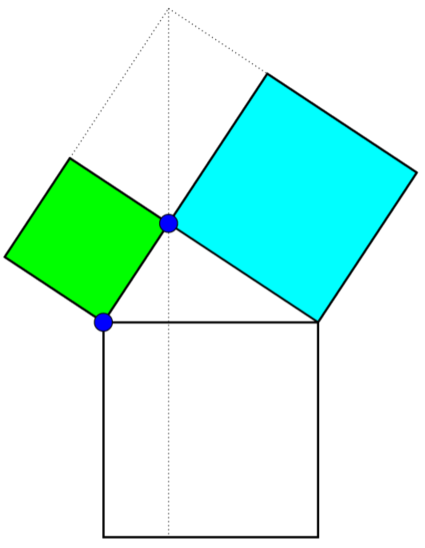
\includegraphics[width=0.5\linewidth]{bilder/Dreieck1.png}
			
			\caption[Grafische Darstellung des SdP I]{Betrachtet wird zunächst die Fläche der beiden Quadrate $a^2$ und $b^2$.}
			\label{fig:fig12}
		\end{minipage}
		\begin{minipage}{0.5\linewidth}
			
			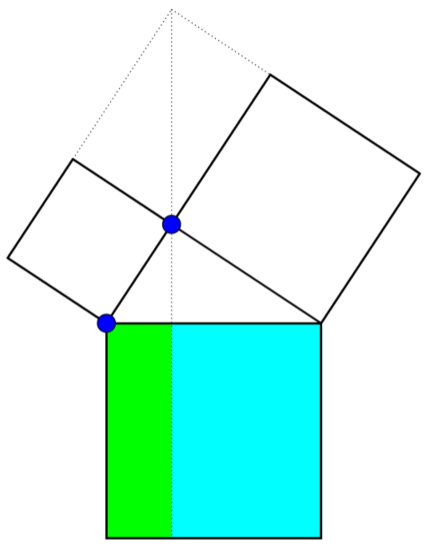
\includegraphics[width=0.49\linewidth]{bilder/Dreieck2.png}
			
			\caption[Grafische Darstellung des SdP I]{Nun werden beide Flächen in das grosse Quadrat mit der Fläche $c^2$. Sie füllen die Fläche aus also gilt die Gleichung. }
			\label{fig:fig13}
		\end{minipage}
	\end{figure} \pagebreak
	\section{Kehrsatz zu Pythagoras}
	\begin{defi}[Kehrsatzz des Pythagoras]
		Wenn in einem Dreieck mit der Hypotenuse $c$ \begin{align}
			a^2+b^2=c^2
		\end{align} gilt, so ist das Dreieck rechtwinklig.
	\end{defi}
	\section{Anwendung des SdP}
	
	\begin{figure}[h]
		\centering
		\begin{minipage}{0.6\linewidth}
			\begin{defi}[Diagonale eines Quadrats]	
				Für ein Quadrat mit der Seitenlänge $a$ beträgt die Diagonale des Quadrats 
				\begin{align}
					d_q^2&=a^2+a^2
					d_q=\sqrt{2a^2}=a\sqrt2
				\end{align}
			\end{defi}
		\end{minipage}
		\begin{minipage}{0.35\linewidth}
		\centering
			\definecolor{ffqqqq}{rgb}{1,0,0}
			\definecolor{yqyqyq}{rgb}{0.5019607843137255,0.5019607843137255,0.5019607843137255}
			\begin{tikzpicture}[line cap=round,line join=round,>=triangle 45,x=1cm,y=1cm,scale=0.7]
				%\draw [color=yqyqyq,, xstep=1cm,ystep=1cm] (-11.66038057704938,-3.3450213874350885) grid (2.5317616952962387,5.902123577473021);
				%\clip(-11.66038057704938,-3.3450213874350885) rectangle (2.5317616952962387,5.902123577473021);
				%\fill[line width=2pt] (-7,3) -- (-7,0) -- (-4,0) -- (-4,3) -- cycle;
				\draw [line width=2pt] (-7,3)-- (-7,0);
				\draw [line width=2pt] (-7,0)-- (-4,0);
				\draw [line width=2pt] (-4,0)-- (-4,3);
				\draw [line width=2pt] (-4,3)-- (-7,3);
				\draw [line width=2pt,color=ffqqqq] (-7,0)-- (-4,3);
			\end{tikzpicture}
			\caption[Quadrat]{Ein Quadrat mit der Seitenlänge $a$ und der Diagonalen $d_q$.}
		\end{minipage}
	\end{figure}
	\begin{figure}[h]
		\begin{minipage}{0.6\linewidth}
			\begin{defi}[Höhe im gleichseitigen Dreieck]
				Für die Höhe $h$ in einem gleichseitigen Dreieck mit der Seitenlänge $a$ gilt
				\begin{align}
					h=\frac{a}{2}\sqrt{3}
				\end{align}
			\end{defi}
		\end{minipage}
		\begin{minipage}{0.3\linewidth}
			\definecolor{ffqqqq}{rgb}{1,0,0}
			\begin{tikzpicture}[line cap=round,line join=round,>=triangle 45,x=1cm,y=1cm, scale=0.7]
				\clip(-9.064463571692091,-2.333956881255677) rectangle (0.38206271465493497,3.8210968314512646);
				%\fill[line width=2pt] (-7,-1) -- (-3,-1) -- (-5,2.4641016151377553) -- cycle;
				\draw [line width=2pt] (-3,-1)-- (-5,2.5);
				\draw [line width=2pt] (-5,2.5)-- (-7,-1);
				\draw [line width=2pt] (-3,-1)-- (-7,-1);
				\draw [line width=2pt,color=ffqqqq] (-5,2.5)-- (-5,-1);
			\end{tikzpicture}
			\caption{Ein Dreieck mit Höhe $h$.}
		\end{minipage}
	\end{figure}
	\begin{figure}[h]
		\begin{minipage}{0.6\linewidth}
			\begin{defi}[Diagonale im Würfel]
				Für die Diagonale $d_w$ eines Würfels mit Kantenlänge $a$ gilt
				\begin{align}
					d_w=\sqrt{d_q^2+a^2}=\sqrt{3a^2+a^2}=a\sqrt{3}
				\end{align}
			\end{defi}
		\end{minipage}
		\begin{minipage}{0.3\linewidth}
			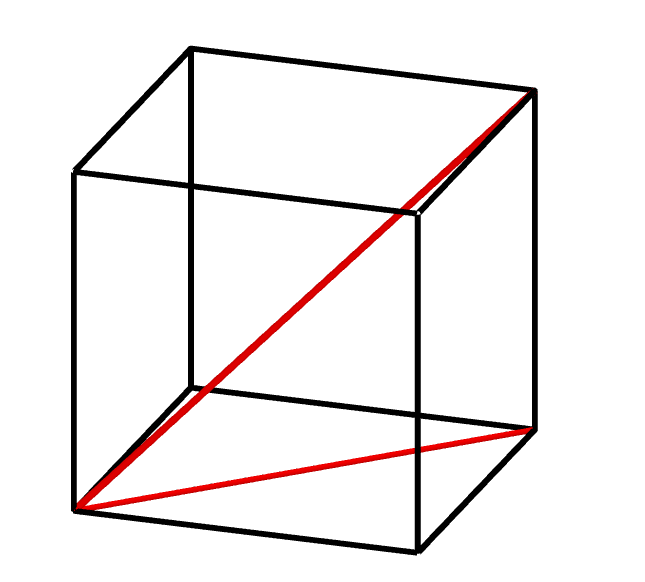
\includegraphics[width=\linewidth]{bilder/würfel.png}
			\caption{Diagonale $d_w$ eines Würfels}
		\end{minipage}
	\end{figure}
	\pagebreak
	\section{Der Kathetensatz}
	\begin{figure}[h]
		\begin{minipage}{0.6\linewidth}
			
	\begin{defi}[Kathetensatz]
		Für jedes rechtwinklige Dreieck gilt:\\
			Das Quadrat über einer Kathete ist flächengleich zum Rechteck aus der Hypotenuse und dem anliegenden Hypotenusenabschnitt.
			\begin{align}
				a^2&=c\x p\\
				b^2&=c \x p
			\end{align}
	\end{defi}
		
		\end{minipage}
		\begin{minipage}{0.4 \linewidth}
		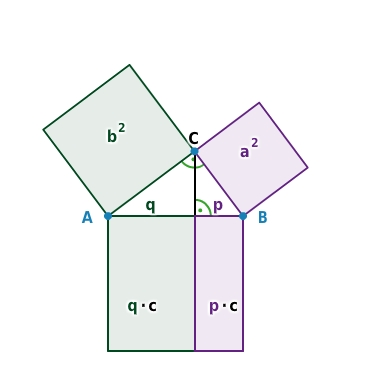
\includegraphics[width=\linewidth]{bilder/ksatz.jpg}
		\caption{Kathetensatz}
		\end{minipage}
	\end{figure}
	\section{Der Höhensatz}
	\begin{figure}[h]
		\begin{minipage}{0.6\linewidth}
			\begin{defi}[Höhensatz]
				Für jedes rechtwinklige Dreieck gilt:\\
				Das Quadrat über der Höhe ist flächengleich zum Rechteck aus den beiden Hypotenusenabschnitten. 
				Es gilt: 
				\begin{align}
					h^2=p \x q
				\end{align}
			\end{defi}
		\end{minipage}
		\begin{minipage}{0.4\linewidth}
			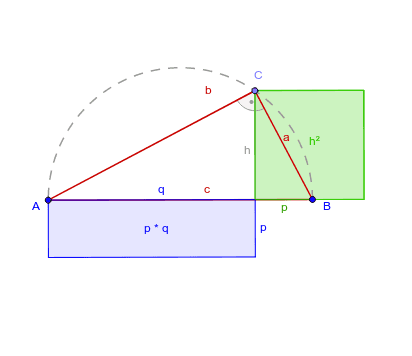
\includegraphics[width=\linewidth]{bilder/hsatz.png}
			\caption{Höhensatz.}
		\end{minipage}
	\end{figure}
	\newpage	
	\chapter{Quadratische Funktionen und Gleichungen}
	\section{Was ist eine quadratische Funktion / Gleichung}
	\begin{defi}[quadratische Funktion / Gleichung]
		Eine Funktion in deren Funktionsterm ein Quadrat vorkommt heisst \textbf{quadratische Funktion}. Sie wird durch den Funktionsterm \eqref{eq:eq7} beschrieben.
		$a,b,c$ sind dabei sog. Parameter, also einfache Zahlenwerte.
		Eine Gleichung ist dann quadratisch, wenn sie die Form \eqref{eq:eq8} annimmt. 
	\end{defi}
	
	\begin{align}
		f(x)&=ax^2+bx+c \label{eq:eq7}\\  0&=ax^2+bx+c \label{eq:eq8}
	\end{align}
	\paragraph{\textsf{Beispiel.}} Für eine Funktion $f(x)=2x^2+4x+12$ ist $a=2,\; b=4, \; c=12$.
	\begin{defi}[(Nomral-) Parabel]
		Der Graph einer quadratischen Funktion heisst \textbf{Parabel}. Der Graph einer Funktion \begin{align}
		y=x^2
	\end{align}
	heisst \textbf{Normalparabel} (s. Abb. \ref{fig:fig8}), da sie der Graph der ''einfachsten`` quadratischen Funktion der Welt ist.
	\end{defi}
	
	\begin{defi}[Scheitelpunkt]
		Der unterste / höchste Punkt bzw. der Punkt an dem sich die Parabel spiegelt heisst \textbf{Scheitelpunkt} $S(x_E\mid y)$ mit $x_E$ als \textbf{Extremstelle}. \footnote{In der Infinitesimalrechnung kann man auch sagen: \textit{Der Scheitelpunkt einer Funktion $y$ ist der Punkt, an dem die Ableitung eine Nullstelle besitzt, also der Punkt einer Parabel mit Steigung 0.}}
	\end{defi}
	
	\begin{figure}[h]
		\centering
		\begin{tikzpicture}[line cap=round,line join=round,>=triangle 45,x=0.5cm,y=0.5cm, scale=0.8]
			\begin{axis}[
				x=0.5cm,y=0.5cm,
				axis lines=middle,
				ymajorgrids=true,
				xmajorgrids=true,
				xmin=-4,
				xmax=4,
				ymin=-2,
				ymax=10,
				xtick={-3,-2,...,3},
				ytick={1,2,...,9},]
				\clip(-8.784290718521506,-3.298627458643907) rectangle (9.521258107057054,10.343530601483076);
				\draw[line width=2pt,smooth,samples=100,domain=-8.784290718521506:9.521258107057054] plot(\x,{(\x)^(2)});
			\end{axis}
		\end{tikzpicture}
		\caption{Graph einer Normalparbel}
		\label{fig:fig8}
	\end{figure}
	\newpage
	\section{Verschiebung von Normalparabeln}
	\subsection{Verschiebung in $y$-Richtung} 
	Eine lineare Funktion $y=mx+t$ lässt sich durch den Parameter $t$, also der ohne Verbindung mit $x$, nach oben / unten verschieben. Ähnlich ist dies auch bei quadratischen Funktionen $y=ax^2+bx+c$. Hier hängt der Parameter $c$ mit keinem $x$, weshalb dieser für die Verschiebung in $y$-Richtung ist.
    Eine quadratische Funktion ist dann in $y$-Richtung Verschoben, wenn der Parameter $c$ geändert wird. (s. Abb. \ref{fig:fig8})
	\begin{defi}[Verschiebung nach oben / unten]
		Eine Funktion, die eine nach oben / unten verschobene Normaplparabel ist, wird immer durch den Funktionsterm
	\begin{align}
		y=x^2+c \label{eq:eq9}
	\end{align}
	beschrieben. Der Scheitelpunkt liegt bei $S(0\mid c)$
	\end{defi}
	\begin{figure}[h]
		\centering
		\definecolor{qqqqff}{rgb}{0,0,1}
		\definecolor{qqwuqq}{rgb}{0,0.39215686274509803,0}
		\begin{tikzpicture}[line cap=round,line join=round,>=triangle 45,x=1cm,y=1cm, scale=0.5]
			\begin{axis}[
				x=1cm,y=1cm,
				axis lines=middle,
				ymajorgrids=true,
				xmajorgrids=true,
				xmin=-6.23229645311294,
				xmax=6.270639702599475,
				ymin=-3.2373404901323446,
				ymax=6.080437025151435,
				xtick={-6,-5,...,6},
				ytick={-3,-2,...,6},]
				\clip(-6.23229645311294,-3.2373404901323446) rectangle (6.270639702599475,6.080437025151435);
				\draw[line width=2pt,color=qqwuqq,smooth,samples=100,domain=-6.23229645311294:6.270639702599475] plot(\x,{(\x)^(2)-2});
				\draw[line width=2pt,smooth,samples=100,domain=-6.23229645311294:6.270639702599475] plot(\x,{(\x)^(2)});
				\draw[line width=2pt,color=qqqqff,smooth,samples=100,domain=-6.23229645311294:6.270639702599475] plot(\x,{(\x)^(2)+1});
			\end{axis}
		\end{tikzpicture}
		\caption[Verschobene Parabeln]{Die Parabeln $f(x)=x^2-2$ (grün), $g(x)=x^2$ (schwarz), $h(x)=x^2+1$ (blau).}
		\label{fig:fig9}
	\end{figure}
	\pagebreak
	\subsection{Verschiebung in $x$-Richtung}
	\begin{figure}[h]
		\begin{minipage}{0.5\linewidth}
			Für die Verschiebung einer Parabel in $x-Richtung$ wird eine neue Art von Funktionsterm \eqref{eq:eq9} in Abhängigkeit eines Parameters $d$ eingeführt\begin{defi}[Verschiebung nach links / rechts]  Diese Form heisst auch \textbf{Scheitelpunktform}.
			\begin{align}
				y=(x+d)^2\Leftrightarrow y=x^2+2dx+d^2 \label{eq:eq5}
			\end{align}
			Hier ist die Parabel um $-d$ nach rechts verschoben (s. Abb. \ref{fig:fig10}). Der Scheitelpunkt liegt dann bei $S(-d\mid 0)$
			\end{defi}
		\end{minipage}
		\begin{minipage}{0.5\linewidth}
			\definecolor{qqqqff}{rgb}{0,0,1}
			\definecolor{qqwuqq}{rgb}{0,0.39215686274509803,0}
			\begin{tikzpicture}[line cap=round,line join=round,>=triangle 45,x=1cm,y=1cm, scale=0.5]
				\begin{axis}[
					x=1cm,y=1cm,
					axis lines=middle,
					ymajorgrids=true,
					xmajorgrids=true,
					xmin=-6.339260735813902,
					xmax=7.304627768708771,
					ymin=-1.44271752481621,
					ymax=7.447202859663722,
					xtick={-6,-5,...,7},
					ytick={-1,0,...,7},]
					\clip(-6.339260735813902,-1.44271752481621) rectangle (7.304627768708771,7.447202859663722);
					\draw[line width=2pt,color=qqwuqq,smooth,samples=100,domain=-6.339260735813902:7.304627768708771] plot(\x,{((\x)-2)^(2)});
					\draw[line width=2pt,smooth,samples=100,domain=-6.339260735813902:7.304627768708771] plot(\x,{(\x)^(2)});
					\draw[line width=2pt,color=qqqqff,smooth,samples=100,domain=-6.339260735813902:7.304627768708771] plot(\x,{((\x)+1)^(2)});
				\end{axis}
			\end{tikzpicture}
			\caption[Verschobene Parabeln]{Die Parabeln $f(x)=(x-2)^2$ (grün), $g(x)=x^2$ (schwarz), $h(x)=(x+1)^2$ (blau).}
			\label{fig:fig10}
		\end{minipage}
	\end{figure}
	%\newpage
	\subsection{Beliebiges Verschieben von Parabeln}
	\begin{defi}[Scheitelpunkt]
		Um Parabeln beliebig zu verschieben muss ein neuer Parameter $e$ zur Scheitelpunktform \eqref{eq:eq10} hinzukommen. Dieser verschiebt um $x$-verschobene Parabeln zusätzlich nach oben/unten.
	Soll die Parabel noch gestreckt bzw. gestaucht werden muss der Parameter $a$ verwendet werden. siehe \eqref{eq:eq11}
	\begin{align}
		y&=(x+d)^2+e=x^2+2dx+d^2+e \label{eq:eq10}\\
		y&=a(x+d^2)+e=ax^2+\underbrace{2adx}_{bx}+\underbrace{ad^2+e}_{c} \label{eq:eq11}
	\end{align}
	\end{defi}
	Um eine Parabel um 3 nach oben und 4 nach rechts zu verschieben, müssen die Parameter $d$ und $e$ geändert werden. (s. Abb. \ref{fig:fig11}) \\
	$d$ verschiebt nach links / rechts $\Rightarrow$ $d=-4$, während $e$ nach oben / unten verschiebt. $\Rightarrow$ $e=3$ Der Funktionsterm ist also 
	\begin{align*}
		y=(x-4)^2+3=x^2-8x+19
	\end{align*}
	\begin{figure}[h]
		\centering
		\definecolor{uuuuuu}{rgb}{0.26666666666666666,0.26666666666666666,0.26666666666666666}
		\definecolor{qqwuqq}{rgb}{0,0.39215686274509803,0}
		\begin{tikzpicture}[line cap=round,line join=round,>=triangle 45,x=0.5cm,y=0.5cm, scale=1]
			\begin{axis}[
				x=0.5cm,y=0.5cm,
				axis lines=middle,
				xmin=-2,
				xmax=8,
				ymin=-1,
				ymax=7,
				xtick={4},
				ytick={3},]
				\clip(-12.526180571954788,-2.070745877770735) rectangle (9.932338139274648,12.56250498982477);
				\draw[line width=1pt,color=qqwuqq,smooth,samples=100,domain=-12.526180571954788:9.932338139274648] plot(\x,{((\x)-4)^(2)+3});
				\draw [line width=1pt,dash pattern=on 1pt off 2pt] (4,3)-- (4,0);
				\draw [line width=1pt,dash pattern=on 1pt off 2pt] (4,3)-- (0,3);
				\draw (1.75,4.25) node[anchor=north ] {$-d$};
				\draw (4.25,2) node[anchor=north west] {$ e$};
				\begin{scriptsize}
					\draw [fill=uuuuuu] (4,3) circle (2pt);
				\end{scriptsize}
			\end{axis}
		\end{tikzpicture}
		\caption[beliebige Verschiebung]{Hier wird die Funktion aus dem Beispiel gezeigt. Diese hat die Parameter $d=-3$ und $e=4$}
		\label{fig:fig11}
	\end{figure}
	\pagebreak
	
	\subsection{Quadratische Ergänzung}
	Es kann vorkommen, dass man den allgemeinen Funktionsterm in die Scheitelpunktform bringen muss:
	\medskip
	
	Wir betrachten also eine Funktion
	\begin{align}
	    f(x)&=ax^2+bx+c,
	\end{align}
	bei der wir zuerst das $a$ ausklammern werden um den Term
	\begin{align}
	    f(x)&=a \left[ x^2+\frac{b}{a}x+ \frac{c}{a} \right]
	\end{align}
	zu erhalten. Im Anschluss versuchen wir die binomischen Formeln (s. Definition \ref{bin:bin-fo}) anzuwenden. Wir brauchen im Mittelteil also etwas, das multipliziert mit 2 $b/a$ ergibt. Dafür erhalten wir $b/2a$.
	\begin{align}
	\begin{aligned}
	    f(x)&=a \left[ x^2+2\x\frac{b}{2a}x+ \frac{c}{a} \right] \\
	    &= a \left[ x^2+2\x\frac{b}{2a}x\underbrace{+\left( \frac{b}{2a}\right)^2-\left( \frac{b}{2a}\right)^2}_{=0} + \frac{c}{a} \right] \\
	    &= a\left[ \left( x+\frac{b}{2a} \right)^2 - \left( \frac{b}{2a}\right)^2+\frac{c}{a} \right]
	\end{aligned}
	\end{align}
	Jetzt muss nur noch $a$ ausklammern:
	\begin{align}
	f(x)&= a\left( x+\frac{b}{2a} \right)^2 - \frac{b}{4a}+c
	\end{align}
	
	Jetzt kann man folgenden Satz definieren:
	\begin{satz}
	Die Extremstelle, also der $x$-Wert des Scheitels, einer quadratischen Gleichung ist bei $x_E=-b/2a$
	\end{satz}
	\begin{proof}
	siehe oben
	\end{proof}
	
	\pagebreak
	\section{Nullstellen und lösen quadratischer Gleichungen}
	\subsection{Funktionen der Form $y=ax^2+bx$}
	Eine Funktion der Form $y=ax^2+bx$ hat die Extremstelle $x_E=\frac{-b}{2a}$ und die Nullstellen $x_1=0$ und $x_2=-\frac ba$, da sich der Funktionsterm zu \eqref{eq:eq12} umformen lässt.
	\begin{align}
		y=ax^2+bx=x(ax+b) \label{eq:eq12}
	\end{align}
	Auf die Schreibweise kann man dann die \textbf{Regel vom Nullprodukt} anwenden.
	\begin{defi}[Regel vom Nullprodukt]
		Die Regel vom Nullprodukt besagt, dass eine Produkt 0 ist, sobald einer der Faktoren null ist.
		\begin{align*}
			p_1=0\lor...\lor p_n=0 \Rightarrow  p=p_1 \x p_2 \x \cdots \x p_n=0 
		\end{align*}
	\end{defi}
	\subsection{Funktionen allgemeiner Form}
	\begin{defi}[Mitternachtsformel]
		Für die Nullstellen einer quadratischen Funktion $y=ax^2+bx+c$ bzw. die Lösung einer quadratischen Gleichung $0=ax^2+bx+c$ gibt es folgende (wichtige) Lösungsformel \eqref{eq:eq15}.
	\begin{align}
		x_{1/2}=\abc \label{eq:eq15}
	\end{align}
	\end{defi}
	\begin{anm}
		 Es gibt immer zwei Lösungen, da $\pm$ bedeutet, dass man $+$ und $-$ rechnet.
	\end{anm} 
	\pagebreak
	\section{Zusatz: Gleichungen mit höheren Potenzen lösen.}
	\begin{defi}[Gleichungen mit Exponenten $e>2$]
	\begin{enumerate}
			\item Eine Gleichung der Form $ax^3+bx^2+cx=0$ kann durch die Regel vom Nullprodukt gelöst werden (s. 3.1).
		\begin{align}
			0=x(ax^2+bx+c).
		\end{align}
		Dann steht in den Klammern eine quadratische Gleichung $0=ax^2+bx+c$ und ausserhalb der Klammer gilt $x=0$.
		\item Eine Gleichung der Form $ax^4+bx^2+c=0$ kann dadurch gelöst werden, dass man ein $u$ definiert für das 
		\begin{align}
			u:=x^2
		\end{align}
		gilt. Setzt man jetzt $u$ ein, so erhält man eine normale quadratische Gleichung mit der Variable $u$. Ist diese gelöst muss man jetzt noch $u$ in $x$ umformen.
		\begin{align}
			u=x^2\Leftrightarrow x=\sqrt u
		\end{align}
	\end{enumerate}
		\end{defi}
	
	\chapter{Quadratische Funktionen in Anwendungen}
	\begin{anm}
		Im folgenden werden typische Aufgabentypen behandelt. Das Wissen um diese Aufgaben zu lösen wurde bereits in vergangen Kapiteln / Schuljahren erlernt. $\Rightarrow$ Es werden nur Lösungsstrategien erarbeitet.
	\end{anm}
	\section{Lineare Gleichungssysteme mit drei Variablen}
	\begin{merk}[Lösungsverfahren von einem LGS]
		Ein lineares Gleichungssystem (LGS) mit drei Gleichungen und drei Variablen \footnote{\textbf{Anmerkung} \quad Ein Gleichungssystem mit drei Variablen und nur zwei Gleichungen lässt sich nicht vollständig lösen.} kann man lösen, indem man es auf ein System mit zwei Gleichungen und zwei Variablen zurückführt.\\
		Dies kann man in den folgenden Schritten machen\footnote{Hier wird das Einsetzungsverfahren beschrieben.}:
		\begin{enumerate}
			\item Eine der drei Gleichungen wird nach einer Variablen aufgelöst.
			\item Aus den beiden andren Gleichungen wird diese Variable durch Einsetzen das sich ergebenden Terms eliminiert.
			\item Das entstehende LGS mit zwei Gleichungen und zwei Variablen wird in der bekannten Weise gelöst.
			\item Den Wer der eliminierten Variablen erhält man durch das Einsetzen der Lösungen in im ersten Schritt aufgelöste Gleichung. 
		\end{enumerate}
	\end{merk}
	\begin{merk}[Fallunterscheidung bei einem LGS]
		Bei einem solchen LGS gibt es drei Fallunterscheidungen:
		\begin{itemize}
			\item Die Gleichungen ergeben drei konkrete Lösungen.
			\item Die Gleichungen sind nach Äquivalenzumformungen identisch. $\Rightarrow$ unendlich viele Lösungen $\Rightarrow$ Man sucht sich eine Variable aus und schreibt die anderen in Abhängigkeit von dieser. 
			\item Die Gleichungen ergeben keine Lösungen.
		\end{itemize}
	\end{merk}
	\subsubsection*{\textsf{Beispiel.}}
	\begin{align*}
		&\text{I)}& 2a-8b+c&=6 \xRightarrow[\text{I'}]{}& c&=8b-2a+6 \\
		&\text{II)}& -a+4b-6c&=-3 \xRightarrow[\text{II'}]{\text{I' in II}}& 6(8b-2a+6)&=4b-a+3 \\
		&&&&11a&=44b+33 \\
		&&&&a&=4b+3\\
		&\text{III)}& 3a-b-c&=20 \xRightarrow[\text{III'}]{\text{I' in III}}& 3a-b-8b+2a+6&=20 \\ 
		&&&&5a-9b&=14 \\
		&&&\xRightarrow[\text{III''}]{\text{II' in III'}}& 5(4b+3)-9b&=14 \\
		&&&&11b&=11 \\
		&&&&b&=1 \\
		&b\, \text{in II')}& a&=4(1)+3=7\\
		&b,a \, \text{in I')}& c&=8(1)-2(7)+6=0 \\
		&&(a,b,z)&=(7,1,0)
	\end{align*}
	\section{Funktionsterm einer quadratischen Funktion ermitteln}
	Um den Funktionsterm einer quadratischen Funktion zu bestimmen gibt es drei Varianten, für die man immer mindestens zwei Punkte braucht.
	\begin{enumerate}
		\item Sind drei beliebige Punkte $P_1(x_1\mid y_1)$, $P_2(x_2\mid y_2)$ und $P_3(x_3 \mid y_3)$, die auf der Parabel liegen, gegeben, so muss man ein LGS aufstellen.
		\begin{align}
			&\text{I)}& y_1&=ax_1^2+bx_1+c \\
			& \text{II)}& y_2&=ax_2^2+bx_2+c \\
			& \text{III)}& y_3&=ax_3^2+bx_3+c
		\end{align}
		Durch Lösen erhält man die Werte für $a$, $b$ und $c$. Damit kann man den Funktionsterm aufstellen.
		\item Ist der Scheitelpunkt $S(x_1\mid y_1)$ und ein (beliebiger) weiterer Punkt $P(x_2\mid y_2)$, so kann man dies in die Scheitlpunktform einsetzen:
		\begin{align}
			f(x)&=a(x-x_1)^2+y_1
		\end{align}
		Um den Parameter $a$ zu bestimmen, muss man nur noch den zweiten Punkt $P$ für $x$ und $f(x)$ einsetzen, sodass man nach $a$ umformen kann.
		\begin{align}
			y_2&=a(x_2-x_1)^2+y_1
		\end{align} 
		\item Sind die Nullstellen $x_1$ und $x_2$ und ein Punkt $P(x_3\mid y_3)$ gegeben so kann man die Nullstellen in die Nullstellenform einsetzen
		\begin{align}
			y&=a(x-x_1)(x-x_2)
		\end{align} 
		Werden jetzt noch die Koordinaten des Punktes eingesetzt, kann man nach $a$ umstellen.
		\begin{align}
			y_3&=a(x_3-x_1)(x_3-x_1)
		\end{align}
	\end{enumerate}

	\pagebreak
	
	\section{Extremwertprobleme}
	
	\begin{anm}
		Extremwertprobleme lassen sich schlecht verallgemeinern, da sie typische Textaufgaben, d.h. sie sind sehr situationsabhängig.
	\end{anm}
	
	Bei Extremwertproblemen will man ein minimales bzw. ein maximales Ergebnis bestimmen. Dabei sind meistens zwei Grössen Gegeben, bei denen die eine von der anderen Abhängig ist:
	\begin{quotation}
		$A$ ist abhängig von $x$ und $y$. Für $x$ gilt meistens: $y =mx+t$. Bestimme $x$ so, dass $A$ möglichst gross / klein ist. \footnote{In der neunten Jahrgangsstufe betrachtet man nur lineare Zuordnungen, da wenn man sie mit der anderen Grösse multipliziert erhält man eine quadratische Funktion: $A(x,y)=xy \Ra A(x)=x(mx+t)=mx^2+tx$}
	\end{quotation}

	Da $A$ (nach Umformung) nur von einer Grösse abhängt, kann man die Extremstelle mit der Formel 
	\begin{align}
		x_E = \frac{-b}{2a}
	\end{align}
	bestimmen und damit $A(x_E)$ berechnen.
	
	\begin{defi}[Extremwertproblem]
		Für die Lösungsmenge eines Extremwertproblems auf eine quadratische Funktion, so ist der Scheitelpunkt die Lösung.
	\end{defi}

	\subsection*{Exkurs: Extremwertprobleme mit anderen Funktionen}
	Die Grösse $A$ wird beschrieben durch $A(x,y)=x+y$, dabei gilt $y = mx+t$. So gilt für $A$: 
	\begin{align}
		A=x+mx+t = x(m+1)+t
	\end{align} Da diese Funktion linear ist, gilt: Umso grösser die $x$ ist, desto grösser ist $A$. Abschliessend kann man sagen:

	\begin{quotation}
		Für streng monotone Funktionen ist der Wert $x_0$ für die Funktion bei $x_0 \to \infty$ am grössten und bei $x_0 \to - \infty$ am kleinsten.
	\end{quotation}

	\pagebreak
	\section{Schnittpunkt bestimmen}
	In diesen Aufgaben ist immer der Schnittpunkt zweier Funktion $f$ und $h$ gesucht. Entweder sind beide Funktionen quadratisch, oder eine ist quadratisch und die andere ist linear.
	
	\begin{defi}[Schnittwertprobleme]
		Ist der Schnittpunkt zweier Funktionen gesucht, so heisst, dass an einem bestimmten $x$-Wert der $y$-Wert beider Funktionen gleich ist. $\Rightarrow$ Setzt man die beiden Funktionen gleich,  \footnote{Man stellt also eine Gleichung auf} so liefert die Lösung dieser Gleichung den $x$-Wert. Der Wert muss dann nur noch in eine der beiden Funktionen eingesetzt werden, und so erhält man den $y$-Wert.
	\end{defi}

	\begin{enumerate}
		\item \textbf{$f$ und $h$ sind quadratische Funktionen} \\
		Herleitung des $x$-Wertes, wenn
		\begin{align}
			f(x)&=ax^2+bx+c \\
			h(x)&=dx^2+ex+f
		\end{align}
		Setzen wir diese beiden Funktionen gleich, so erhält man folgende Lösungsmenge für $x$:
		\begin{align}
			\begin{aligned}
			ax^2+bx+c &= dx^2+ex+f \\
			0 &= (a-d)x^2+(b-e)x+(c-f) \\
			x &= \frac{-(b-e)\pm \sqrt{(b-e)^2-4(a-d)(c-f)}}{2(a-d)}
			\end{aligned}
		\end{align}
		
		Nun kann man $x$ in $f(x)$ oder in $h(x)$ einsetzen und erhält den Schnittpunkt.
		
		\begin{anm}
			Auch hier spielt die Diskriminante eine Rolle, sie entscheidet darüber, wie viele Schnittpunkte die Parabeln haben. 
		\end{anm}
		
		\item \textbf{$f$ ist eine quadratisache und $h$ ist eine lineare Funktion} \\
		
		\begin{align}
		    f(x)&=ax^2+bx+c \\ 
		    g(X)&=dx+e
		\end{align}
		Auch hier setzt man die beiden Term wiedergleich
	\end{enumerate}

    \chapter{Wahrschinlichkeit bei mehrstufigen Zufallsexperimenten}
    \section{Mehrstufige Zufallsexperimente}
\begin{defi}
    Besteht ein Zufallsexperiment aus mehreren geordneten  Teilexperimenten, so ist es ein \textbf{mehrstufiges Zufallsexperiment.}
\end{defi}


Kommt es auf die Reihenfolge an, so schreibt man die möglichen Ergebnisse als Paare $(a_1;a_2)$, als Tripel $(a_1;a_2;a_3)$ oder allgemein als $n$-Tupel $(a_1;...;a_n)$. 
Da eine Menge an Tupeln unübersichtlich werden kann, zeichnet man Baumdiagramm zur Veranschaulichung.

    \begin{bsp} \label{bsp:bsp51}
    Für den Münzwurf gibt es zwei Ereignisse: \textit{Kopf} ({k}) und \textit{Zahl} ({z}). Wirft man die Münze zweimal, so gibt es folgende Möglichkeiten: \begin{align}
        \Omega = \{ (k;k), (k;z), (z;k), (z;z) \}
    \end{align}
    Links in Abb. \ref{fig:51} sieht man den Baum und rechts sieht man das Ereignis $A:$ ``zweimal Kopf'' in rot: $A=\{(k;k)\}$.
    \end{bsp}   

\begin{figure}[h]
    \begin{minipage}{0.5\linewidth}
    \centering
    \begin{forest}
        [ [\textsf k [\textsf k ] [\textsf z] ] [\textsf z [\textsf k ] [\textsf z] ] ]
    \end{forest}
    \end{minipage}
    \begin{minipage}{0.5\linewidth}
    \centering
    \begin{forest}
        [ [\red \textsf k, edge = red [\red \textsf  k  , edge = red] [\textsf z] ] [\textsf z [\textsf k ] [\textsf z] ] ]
    \end{forest}
    \end{minipage}
    
    \caption{Baumdiagramm zu Bsp. \ref{bsp:bsp51}}
    \label{fig:51}
\end{figure}
\pagebreak
\begin{bsp} \label{bsp:bsp52}
    Bei einem Galton-Brett fällt eine Kugel durch ein Brett mit Zapfen. An jedem Zapfen wird sei entweder nach links (l) oder rechts (r) abgelenkt. 
    \begin{enumerate}[wide=0em, leftmargin=*, label=(\alph*), itemsep=0pt, parsep=0pt]
        \item Bestimme für die ersten drei Ablenkungen alle möglichen Ergebnisse mit Hilfe eines Baumdiagramms.
        \item Gib das Ergebnis, in das Fach B zu fallen, als Menge von Ereignissen an. \footnote{siehe Abbildung auf \url{http://www.lukas-semrau.de/galton}. Gemeint ist Spalte (1).}
    \end{enumerate}
\end{bsp}

\begin{proof}[Lösung zu Beispiel \ref{bsp:bsp52}.]
\begin{enumerate}[label = \alph*)]
    \item Baumdiagramm s. Abb. \ref{fig:52} 
    \begin{figure}[h]
        \centering
        \begin{forest}
            [[\sf l[\sf l[\sf l][\sf r]][\sf r[\sf l][\sf r]]][\sf r[\sf l[\sf l][\sf r]][\sf r[\sf l][\sf r]]]]
        \end{forest}
        \caption{Baumdiagramm zu (\ref{bsp:bsp52}a)}
        \label{fig:52}
    \end{figure}
    \item Alle Ergebnisse für $B=$ Die Kugel fällt in dass Fach B.
    \begin{align}
        B = \{(l;l;l), (l;r;l), (r;l;l) \}
    \end{align}
\end{enumerate}
\end{proof}

\section{Pfadregeln}
\subsection{erste Pfadregel}

\begin{defi}[1. Pfadregel / Produktregel]
Die Wahrscheinlichkeit eines Ereignisses erhält man indem man die Wahrscheinlichkeiten pro Pfad (der zum jeweiligen Ereignis hinführt) im Baumdiagramm multipliziert.
\end{defi}
\begin{merk}
Die Summe aller Wahrscheilichkeiten beträgt immer 1.
\begin{align}
    P(\Omega)=1
\end{align}
\end{merk}

\chapter{Trigonometrie}

\section{Verhältnisse im rechtwinkligen Dreieck}

\begin{figure}[h]
    \centering
    \definecolor{qqqqff}{rgb}{0,0,1}
\definecolor{qqwuqq}{rgb}{0,0.39215686274509803,0}
\definecolor{ccqqqq}{rgb}{0.8,0,0}
\begin{tikzpicture}[line cap=round,line join=round,>=triangle 45,x=1cm,y=1cm]
\clip(-0.5,-0.5) rectangle (5.5,2.5);
\draw[line width=2pt,color=ccqqqq,fill=ccqqqq,fill opacity=0.1] (3.7367336268050644,1.8683668134025322) -- (3.8683668134025324,1.6051004402075968) -- (4.131633186597468,1.7367336268050646) -- (4,2) -- cycle; 
\draw [shift={(5,0)},line width=2pt,color=qqwuqq,fill=qqwuqq,fill opacity=0.10000000149011612] (0,0) -- (116.56505117707799:0.5676282072462927) arc (116.56505117707799:180:0.5676282072462927) -- cycle;
\draw [shift={(0,0)},line width=2pt,color=qqqqff,fill=qqqqff,fill opacity=0.1] (0,0) -- (0:0.7568376096617235) arc (0:26.56505117707799:0.7568376096617235) -- cycle;
\draw [line width=2pt] (0,0)-- (4,2);
\draw [line width=2pt] (4,2)-- (5,0);
\draw [line width=2pt] (5,0)-- (0,0);
\draw (2.7112468590079843,-0.017280080088737635) node[anchor=north west] {$c$};
\draw (2.3,1.8) node[anchor=north west] {$b$};
\draw (4.565499002679207,1.3677327455922141) node[anchor=north west] {$a$};

\draw (3.6,1.6) node[anchor=north west] {$\gamma$};
\draw (4.1,0.65) node[anchor=north west] {$\beta$};
\draw (0.7,0.4) node[anchor=north west] {$\alpha$};
\begin{scriptsize}
\draw [fill=black] (0,0) circle (1.5pt) node [left] {\large $A$};
\draw [fill=black] (4,2) circle (1.5pt) node [above] {\large $C$};
\draw [fill=black] (5,0) circle (1.5pt) node [right] {\large $B$};
\end{scriptsize}
\end{tikzpicture}
    \caption{Betrachtete Dreiecke}
    \label{fig:fig61}
\end{figure}

Wir betrachten die rechtwinklige Dreiecke (vgl. Abb. \ref{fig:fig61}) bei denen $\alpha$ bei $A$, $\beta$ bei $B$ und $\gamma$ bei $C$ liegt. Die Seite $a$ liegt dann gegenüber von $A$, die Seite $b$ gegenüber von $B$ und $c$ gegenüber von $C$.

Die Begriffe Kathete und Hypotenuse sind aus der 7. Klasse bereits bekannt, dennoch werden sie hier nochmals definiert:
\begin{itemize}
    \item Die Hypotenuse ($HY$) ist die Seite, die gegenüber des rechten Winkels liegt.
    \item Die Katheten sind die Seiten, die am rechten Winkel liegen.
\end{itemize}

\begin{defi}[Ankathete und Gegenkathete]
Betrachten wird der Winkel $\alpha$, so ist die Ankathete zu $\alpha$ ($AK_\alpha$) die Seite $b$, da sie an dem Winkel $\alpha$ liegt. Die Gegenkathete zu $\alpha$ ($GK_\alpha$) ist dann die Seite $a$, da sie gegenüber von $\alpha$ liegt.
\end{defi}

Sind die Seitenverhältnisse im Dreieck bekannt, so kann man die BEgriffe ``Sinus'', ``Kosiunus'' und ``Tangens'' einführen.

\begin{defi}
    \begin{align}
    \sin \alpha &= \frac{GK_\alpha}{HY} & \textsf{(Sinus (von) Alpha)} \\
    \cos \alpha &= \frac{AK_\alpha}{HY} & \textsf{(Kosinus (von) Alpha)} \\
    \tan \alpha &= \frac{GK_\alpha}{AK_\alpha} & \textsf{(Tangens (von) Alpha)}
    \end{align}
\end{defi}
\pagebreak
\paragraph{\textsf{Beispielaufgabe.}} Betrachtet wird ein Dreieck aus Abb. \ref{fig:fig61}, bei dem $\gamma$ der rechte Winkel ist, die Hypotenuse $c = 4$ und der Winkel $\alpha=60^\circ$ Bestimme $a$ und $b$.
\begin{losung}
Es gilt:
\begin{align}
    \begin{aligned}
    \sin 60^\circ &= \frac{a}{4} \\
    \Leftrightarrow a &= \sin 60^\circ \x 4 \\
    &= 2\sqrt{3}\approx 3.46\\
    \cos 60^\circ &= \frac{b}{4} \\
    \Leftrightarrow b &= \cos 60^\circ \x 4 \\
    &= 2
    \end{aligned}
\end{align}
\end{losung}

\section{Sinus, Kosinus und Tangens am Einheitskeis.}

\begin{defi}[Einheitskreis]
Ein Einheitskreis ist ein Kreis mit $r = 1$.
\end{defi}

\begin{figure}[h]
    \centering
    \begin{tikzpicture}[scale=2,cap=round]
% Local definitions
\def\costhirty{0.8660256}
% Colors
\colorlet{anglecolor}{green!50!black}
\colorlet{sincolor}{red}
\colorlet{tancolor}{orange!80!black}
\colorlet{coscolor}{blue}
% Styles
\tikzstyle{axes}=[]
\tikzstyle{important line}=[very thick]
\tikzstyle{information text}=[rounded corners,fill=red!10,inner sep=1ex]
% The graphic
\draw[style=help lines,step=0.5cm] (-1.4,-1.4) grid (1.4,1.4);
\draw (0,0) circle (1cm);
\begin{scope}[style=axes]
\draw[->] (-1.5,0) -- (1.5,0) node[right] {$x$} coordinate(x axis);
\draw[->] (0,-1.5) -- (0,1.5) node[above] {$y$} coordinate(y axis);
\foreach \x/\xtext in {-1, -.5/-\frac{1}{2}, 1}
\draw[xshift=\x cm] (0pt,1pt) -- (0pt,-1pt) node[below,fill=white] {$\xtext$};
\foreach \y/\ytext in {-1, -.5/-\frac{1}{2}, .5/\frac{1}{2}, 1}
\draw[yshift=\y cm] (1pt,0pt) -- (-1pt,0pt) node[left,fill=white] {$\ytext$};
\end{scope}
\filldraw[fill=green!20,draw=anglecolor] (0,0) -- (3mm,0pt) arc(0:30:3mm);
\draw (15:2mm) node[anglecolor] {$\alpha$};
\draw[style=important line,sincolor]
(30:1cm) -- node[left=1pt,fill=white] {$\sin \alpha$} (30:1cm |- x axis);
\draw[style=important line,coscolor]
(30:1cm |- x axis) -- node[below=2pt,fill=white] {$\cos \alpha$} (0,0);
\draw[style=important line,tancolor] (1,0) -- node[right=1pt,fill=white] {
$\displaystyle \tan \alpha \color{black}=
\frac{{\color{sincolor}\sin \alpha}}{\color{coscolor}\cos \alpha}$}
(intersection of 0,0--30:1cm and 1,0--1,1) coordinate (t);
\draw (0,0) -- (t);
\end{tikzpicture}
    \caption{Sinus, Kosinus und Tangens am Einheitskreis.}
    \label{fig:62}
\end{figure}

\paragraph{\textsf{Erklärung zu Abb. \ref{fig:62}}}
Wir betrachten ein Dreieck in dem die Hypotenuse der Radius $r=1$ ist, betrachten wir den Winkel $\alpha$, so gilt für Kosinus und Sinus:

\begin{align}
    \begin{aligned}
    \sin \alpha &= \frac y1 \\ &= y \\
    \cos \alpha &= \frac{x}{1} \\ &= x
    \end{aligned}
\end{align}

Betrachtet man den Sinus als Funktion die jedem Wert $\alpha \in \left[ 0^\circ : 90^\circ \right]$ ein $\alpha \mapsto \sin \alpha$ zuordnet, stellt man fest dass der Wert vom Sinus wischen 0 und 1 liegt: \\ \begin{center}
    $\sin 0^\circ = 0$ und $\sin 90^\circ = 1$
\end{center}

Wird jedem $\alpha$ nun $\alpha \mapsto \cos \alpha$ zugeordnet, stellt man fest, dass der Funktionswert zwischen 1 und 0 liegt:
\\ \begin{center}
    $\cos 0^\circ = 1$ und $\sin 90^\circ = 0$
\end{center}

\subsection{Umkehrfunktion von Sinus, Kosinus und Tangens}

Kennt man den Wert $x$, den $\sin \alpha = x$ besitzt, dann kann man mit der Umkehrfunktion des Sinus $\arcsin$\footnote{oft verwendet man die Notation $\sin^{-1}$, die ich aber nicht verwenden möchte da $\sin^{-1}x \neq 1/\sin x$ aber $\sin^2x = \sin x \x \sin x $ ist.} herausfinden, wie groß $\alpha$ ist.
\begin{align}
    \arcsin\left( \frac{GK_\alpha}{HY} \right) &= \alpha \\
    \arccos\left( \frac{AK_\alpha}{HY} \right) &= \alpha\\
    \arctan\left( \frac{GK_\alpha}{AK_\alpha} \right) &= \alpha
\end{align}

\section{Beziehungen zwischen Sinus, Kosinus und Tangens}
\begin{satz}
$\sin^2x+\cos^2x=1$
\end{satz}
\begin{proof}
\begin{align}
    \begin{aligned}
    \sin^2x+\cos^2x &= \frac{GK_x^2}{HY^2}+\frac{AK_x^2}{HY^2} \\ 
    &= \frac{GK_x^2+AK_x^2}{HY^2}
    \end{aligned}
\end{align}

\begin{lemma}[Satz des Pythagoras]
    Nach dem SdP gilt: $GK_x^2+AK_x^2 = HY^2$
\end{lemma}
\begin{align}
    \begin{aligned}
    \sin^2x+\cos^2x &= \frac{HY^2}{HY^2}\\
    &= 1
    \end{aligned}
\end{align}
\end{proof}

\begin{satz}
$\tan x = \sin x / \cos x$
\end{satz}

\begin{proof}
\begin{align}
    \begin{aligned}
    \frac{\sin x}{\cos x} &= \frac{\;\frac{GK_x}{HY}\;}{\frac{AK_x}{HY}} \\ &= \frac{GK_x \x HY}{AK_x \x HY}
    \\ &= \frac{GK_x}{AK_x}=\tan x
    \end{aligned}
\end{align}
\end{proof}

\pagebreak

\begin{satz}\label{satz:4}
Der Satz besteht aus zwei Teilen.
\begin{enumerate}
    \item $\sin \alpha = \cos(90^\circ - \alpha)$
    \item $\cos \alpha = \sin(90^\circ -\alpha)$
\end{enumerate}
\end{satz}
\begin{proof}
\begin{figure}[h]
    \centering
    \begin{tikzpicture}[line cap=round,line join=round,>=triangle 45,x=1cm,y=1cm]
\begin{axis}[
x=1cm,y=1cm,
axis lines=middle,
xmin=-1,
xmax=5,
ymin=-1,
ymax=4,
xtick=\empty,
ytick=\empty,
xlabel={$x$ },
ylabel={$y$ }]
\clip(-4.024073913258687,-3.141530445200277) rectangle (7.071204292300675,4.087797166087527);
\draw [line width=2pt,color=qqwuqq] (0,0)-- (4,0);
\draw [line width=2pt,color=qqqqff] (4,3)-- (4,0);
\draw [line width=2pt,color=qqwuqq] (4,3)-- (0,3);
\draw [line width=2pt,color=qqqqff] (0,3)-- (0,0);
\draw [line width=2pt,color=ffqqtt] (4,3)-- (0,0);
  \draw
    (4,0) coordinate (a) %node[right] {a}
     (0,0) coordinate (b) %node[left] {b}
     (4,3) coordinate (c) %node[above right] {c}
    pic["$\alpha$", draw=black,line width = 1pt, -, angle eccentricity=1.2, angle radius=1cm]
    {angle=a--b--c};

  \draw
    (4,3) coordinate (a) %node[right] {a}
     (0,0) coordinate (b) %node[left] {b}
     (0,3) coordinate (c) %node[above right] {c}
    pic["$90^\circ - \alpha$", draw=black,line width = 1pt, - -, angle eccentricity=1.2, angle radius=1.5cm]
    {angle=a--b--c};
    \draw
    (4,0) coordinate (a) %node[right] {a}
     (0,0) coordinate (b) %node[left] {b}
     (0,3) coordinate (c) %node[above right] {c}
    pic["", draw=black,line width = 0.5pt, - -, angle eccentricity=1.2, angle radius=0.5cm]
    {angle=a--b--c};
    \node[] at (-0.5,0.25) {$90^\circ$};
    \draw [line width=0.5pt,color=black] (-0.25,0.25)-- (0.25,0.25) ;
    \node[rotate = 90, color = qqqqff] at (-0.24, 1.5) {$AK_{90^\circ - \alpha}$};
    \node[ color = qqqqff] at (4.5, 1.5) {$GK_{\alpha}$};
    \node[ color = qqwuqq] at (2, 3.25) {$GK_{90^\circ - \alpha}$};
    \node[ color = qqwuqq] at (2, -0.25) {$AK_{\alpha}$};
\end{axis}
\end{tikzpicture}
    \caption{Abb. zum Beweis von Satz \ref{satz:4}}
    \label{fig:63}
\end{figure}
In Abb. \ref{fig:63} sieht man das folgende Seiten gleich sind.
\begin{align}
    \begin{aligned}
    GK_\alpha &= AK_{90^\circ - \alpha}\\
    AK_\alpha &= GK_{90^\circ - \alpha}
    \end{aligned} \label{eq:634}
\end{align}

Jetzt muss man sich nur noch überlegen, die Verhältnisse überlegen:
\begin{align}
    \sin \alpha &= \frac{GK_\alpha}{HY} \\ 
    \cos \alpha &= \frac{AK_\alpha}{HY} \\
    \sin(90^\circ - \alpha) &= \frac{GK_{90^\circ - \alpha}}{HY} \\
    \cos(90^\circ - \alpha) &= \frac{AK_{90^\circ - \alpha}}{HY}
\end{align}
Aus \eqref{eq:634} kann man nun folgern, dass 
\begin{align}
    \sin \alpha = \frac{GK_\alpha}{HY} &= \frac{AK_{90^\circ - \alpha}}{HY} = \cos(90^\circ - \alpha) \\
    \cos \alpha = \frac{AK_\alpha}{HY} &= \frac{GK_{90^\circ - \alpha}}{HY} = \sin(90^\circ - \alpha)
\end{align}
\end{proof}

\chapter{Raumgeometrie}
\section{Geraden und Ebenen im Raum}

\begin{defi}[Lot]
Eine Gerade $s$ heisst \textbf{Senkrechte (Lot)} zur Ebene $E$, wenn sie mit zwei (beliebigen) Punkten Geraden $g$ und $h$ dieser Ebene $E$, die durch den Schnittpunkt $F$ gehen, einen rechten Winkel bildet.
\end{defi}

\end{document}